\documentclass{beamer}
\usepackage[T1]{fontenc}
\usepackage[utf8]{inputenc}
\usepackage{lmodern}
\usepackage[francais]{babel}
\usepackage{graphicx}
\usepackage{beamerthemeWarsaw}
\expandafter\def\expandafter\insertshorttitle\expandafter{\insertshorttitle\hfill\insertframenumber\,/\,\inserttotalframenumber}

\title{Projets Test - Groupe 6}
\author{Kevin \textsc{Boulala}, Maxime \textsc{Dubois}}
\institute{Université de Franche Comté}
\date{\today}

\begin{document}

  \begin{frame}
    \titlepage
  \end{frame}

  \begin{frame}
    \setcounter{tocdepth}{2}
	  \tableofcontents[]
  \end{frame}
  
  \section{Développeur}
  
    \begin{frame}
    	\tableofcontents[currentsection]
    \end{frame}
  
    \subsection{Présentation de Mark Attacks}
    \begin{frame}
      \frametitle{Mark Attacks}
      \begin{block}{}
        \begin{itemize}
          \item Pour les enseignants et les étudiants
          \item Saisir les notes et les afficher
          \item Gestion des modules
          \item Mais aussi des statistiques diverses
        \end{itemize}
      \end{block}
    \end{frame}
    
    \subsection{Les fonctionnalités développées et non développées}
    \begin{frame}
      \frametitle{Les fonctionnalités développées}
      \begin{block}{}
        \begin{itemize}
          \item Gestion des enseignants - Ajout
          \item Gestion des étudiants - Ajout
          \item Gestion des UE - Ajout
          \item Gestion des UE - Suppresion des modules
          \item Connexion de l'administrateur, d'un étudiant, d'un enseignant
          \item Validation : login, mot de passe, prénom, nom, adresse, date de naissance, mail, téléphone, description, code module, titre module
          \item Site résistant aux attaques
          \item Navigation du site (sur divers navigateurs)
          \item Navigation mobile
        \end{itemize}
      \end{block}
    \end{frame}
    \begin{frame}
      \frametitle{Les fonctionnalités non développées 1/4}
      \begin{block}{}
        \begin{itemize}
          \item Gestion des enseignants - Recherche
          \item Gestion des enseignants - Approbation compte
          \item Gestion des enseignants - Suppression
          \item Gestion des enseignants - Modification
          \item Gestion des étudiants - Modification
          \item Gestion des etudiants - Recherche
          \item Gestion des etudiants - Approbation compte
          \item Gestion des etudiants - Suppression
          \item Gestion des UE - Modifier module
          \item Gestion des modules - Recherche
        \end{itemize}
      \end{block}
    \end{frame}
    \begin{frame}
      \frametitle{Les fonctionnalités non développées 2/4}
      \begin{block}{}
        \begin{itemize}
          \item Gestion des modules - Affectation
          \item Gestion des enseignants - Approbation module
          \item Ajout d'autres enseignants
          \item Recherche d'étudiants
          \item Accès des informations
          \item Ajout d'étudiants
          \item Suppression d'enseignants
          \item Gestion des notes
          \item Modification des notes
          \item Ajout du coefficient du module
        \end{itemize}
      \end{block}
    \end{frame}
    \begin{frame}
      \frametitle{Les fonctionnalités non développées 3/4}
      \begin{block}{}
        \begin{itemize}
          \item Modification du coefficiant du module
          \item Suppression des notes
          \item Reset password
          \item Demande de compte enseignant, étudiant
          \item Espace utilisateur - Connexion
          \item Espace utilisateur - Consulation des stats recapitulatives
          \item Espace utilisateur - Consulation des notes
          \item Espace utilisateur - Consulation des stats
          \item Description compte utilisateur
          \item Changement des informations personnelles
        \end{itemize}
      \end{block}
    \end{frame}
    \begin{frame}
      \frametitle{Les fonctionnalités non développées 4/4}
      \begin{block}{}
        \begin{itemize}
          \item Description d'un module
          \item Notifications
          \item Liste des référents
          \item Notifications administrateur, enseignant, étudiant
        \end{itemize}
        \begin{center}
          Voilà.
        \end{center}
      \end{block}
    \end{frame}
    \begin{frame}
      \frametitle{Bilan à propos des fonctionnalités}
      \begin{block}{Les fonctionnalités développées}
        \begin{center}
          21 exigences développées
        \end{center}
      \end{block}
      \begin{block}{Les fonctionnalités non-développées}
        \begin{center}
          35 exigences non-développées
        \end{center}
      \end{block}
    \end{frame}

    \subsection{Démonstration}
    \begin{frame}
      \frametitle{Démonstration}
      \begin{center}
        {\LARGE Lançons \href{http://localhost/m2test6/markattaks-tmp/website/}{Mark Attacks}}
      \end{center}
    \end{frame}
    
    \subsection{Synthèse du travail réalisé}
    
      \subsubsection{Infrastructure}
      \begin{frame}
        \frametitle{Infrastructure}
        \begin{block}{}
          \begin{itemize}
            \item Pour les exigences et les cas de tests : \textbf{Squash TM}
            \item Gestion de production : pas Maven, mais \textbf{Gradle}
            \item Gestionnaire de versions : \textbf{SVN}
            \item Intégration continue : \textbf{Jenkins}
          \end{itemize}
        \end{block}
      \end{frame}
      
      \subsubsection{Tests d'acceptation}
      \begin{frame}
        \frametitle{Tests d'acceptation}
        \begin{block}{Pour quoi faire ?}
          Pour s'assurer du comportement attendu de l'application. Il faut pour cela comparer le comportement de l'application livrée à ce qui est indiqué dans Squash TM, notamment dans les cas de tests.
        \end{block}
        \begin{block}{Couverture}
          Toutes les fonctionnalités développées sont testées, à l'exception de :
          \begin{itemize}
            \item La taille du nom des modules lors d'un ajout de module par l'administrateur
          \end{itemize}
        \end{block}
      \end{frame}
      
      \subsubsection{Tests d'intégration}
      \begin{frame}
        \frametitle{Tests d'intégration}
        \begin{block}{Pour quoi faire ?}
          Pour s'assurer du bon comportement de l'application en général.
          \begin{itemize}
            \item Est-ce qu'un utilisateur qui a ce statut peut accéder à toutes les pages ?
            \item Est-ce que l'icône des notifications apparaît après s'être connecté ?
            \item Est-ce que lorsqu'on ajoute un utilisateur, il s'ajoute bien dans la liste des utilisateurs ?
            \item Etc
          \end{itemize}
        \end{block}
      \end{frame}
      \begin{frame}
        \frametitle{Tests d'intégration}
        \begin{block}{Taux de recouvrement}
          \begin{columns}
            \begin{column}{.6\textwidth}
              \begin{center}
                \scalebox{0.4}{
                  \begin{tabular}{|l|cc|}
                    \hline
                    Exigences & Nb tests &	Etat des tests \\
                    \hline
                    Gestion des enseignants - Ajout	& 7 &	Pass \\
                    Gestion des étudiants - Ajouts	& 7 &	Pass  \\
                    Gestion des UE - Ajout	& 7 &	Pass  \\
                    Gestion des UE - Suppresion des modules	& 1 &	Pass  \\
                    Connexion de l'administrateur	& 4 &	Pass  \\
                    Connexion d'un étudiant	& 4 &	Pass  \\
                    Connexion d'un enseignant	& 4 &	Pass  \\
                    Validation - Mot de passe	& 1 &	Pass  \\
                    Validation - Login	& 1 &	Pass  \\
                    Validation - Prénom	& 7 &	Pass  \\
                    Validation -  Nom	& 7 &	Pass  \\
                    Validation - Adresse	& 7 &	Pass  \\
                    Validation - Date de naissance	& 7 &	Pass  \\
                    Validation - mail	& 7 &	Pass  \\
                    Validation - téléphone	& 7 &	Pass  \\
                    Description	& 2 &	Pass  \\
                    Code Module	& 2 &	Pass  \\
                    Titre	& 0 &	-  \\
                    Site résistant aux attaques	& 0 &	-  \\
                    Navigation du site	& 0 &	Manuel  \\
                    Navigation mobile	& 0 &	Manuel  \\
                    \hline
                  \end{tabular}
                }
              \end{center}
            \end{column}
            \begin{column}{.4\textwidth}
              \begin{itemize}
                \item {\scriptsize Rappel : 21 exigences développées}
                \item {\scriptsize 17 testées auto}
                \item {\scriptsize 2 testées manuellement}
                \item {\scriptsize 2 non testées}
              \end{itemize}
              Taux de recouvrement \textbf{90,47\%}
            \end{column}
          \end{columns}
        \end{block}
      \end{frame}
      \begin{frame}
        \frametitle{Tests d'intégration}
        \begin{block}{Exemple : Gestion des étudiants - Ajouts}
          \begin{columns}
            \begin{column}{.5\textwidth}
              \begin{center}
                \begin{tiny}
                  LOGIN = "Albator"\\
                  LOGIN2 = "Kakarot"\\
                  PW\_OK = "Azerty08"\\
                  PW\_OK2 = "Qwerty08"\\
                  PW\_TOO\_SHORT = "Azer867"\\
                  PW\_WITHOUT\_LOW = "AZERTY08"\\
                  PW\_WITHOUT\_UP = "azerty08"\\
                  PW\_WITHOUT\_NUM = "azertyAA"\\
                  FN = "David"\\
                  LN = "Hasselhoff"\\
                  DATE\_OK = "1952-02-21"\\
                  DATE\_OK\_LIMITE = "1876-01-01"\\
                  DATE\_NOK\_LIMITE = "1875-12-31"\\
                  ADDRESS = "55 rue du Faubourg-Saint-Honoré"\\
                  PHONE\_OK = "0123456789"\\
                  PHONE\_TOO\_LONG = "01234567890"\\
                  PHONE\_TOO\_SHORT = "012345678"\\
                  PHONE\_WRONG\_FORMAT = "0123aaa789"\\
                  MAIL\_OK = "coucou.titou@mail.com"\\
                  MAIL\_OK2 = "adresse@mail.com"\\
                  MAIL\_NOK = "coucou.titou\_mail.com"\\
                \end{tiny}
              \end{center}
            \end{column}
            \begin{column}{.5\textwidth}
              \begin{center}
                \begin{small}
                  testAddUserSuccess\\
                  testAdd2UsersSameLogin\\
                  testAddUserIncorrectPassword\\
                  testAddUserBirthDateLimits\\
                  testAddUserIncorrectPhoneNumber\\
                  testAddUserIncorrectMail\\
                  testAdd2UsersSameMail\\
                \end{small}
              \end{center}
            \end{column}
          \end{columns}
        \end{block}
      \end{frame}
      
      \subsubsection{Tests unitaires}
      \begin{frame}
        \frametitle{Tests unitaires}
        \begin{block}{Pour quoi faire ?}
          Pour s'assurer du bon comportement des fonctions. Qu'est-ce que nous avons testé ?
          \begin{itemize}
            \item La base de donnée : se connecter, la réinitiailiser
            \item Le modèle de donnée : insertion, suppression, trouver un enregistrer ou un ensemble d'enregistrements
            \item Les fonctions développées
            \item Etc
          \end{itemize}           
        \end{block}      
      \end{frame}
      \begin{frame}
        \frametitle{Tests unitaires}
        \begin{block}{Taux de recouvrement et structure}
          \begin{figure}
            \begin{center}
              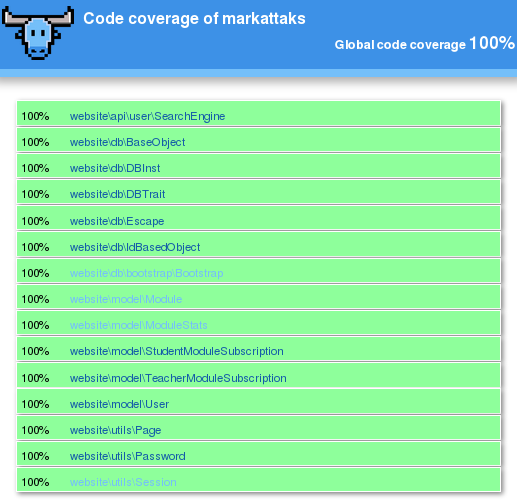
\includegraphics[width=.5\textwidth]{images/atoum.png}
              \label{fig:cov_tu}
            \end{center}
          \end{figure}
        \end{block}
      \end{frame}
      
      \subsubsection{Bilan des problèmes et de leurs solutions}
      \begin{frame}
        \frametitle{Bilan des problèmes}
        \begin{block}{}
          \begin{itemize}
            \item Quelques soucis liés aux outils (VPN, Squash TM, Jenkins)
            \item Un temps de chauffe qui a englouti le Sprint 1
          \end{itemize}
        \end{block}
      \end{frame}
      
    \subsection{Synthèse du travail en équipe}
      
      \subsubsection{Organisation de l'équipe}
      \begin{frame}
        \frametitle{Organisation de l'équipe}
        \begin{block}{C'est simple...}
          ... ce que tu développes, tu le testes.\\
          L'autre développeur jète un oeil au travail fourni avant de valider la tâche.
        \end{block}
      \end{frame}
      
      \subsubsection{Les évolutions au cours du projet}
      \begin{frame}
        \frametitle{Les évolutions au cours du projet}
        \begin{block}{Très peu d'évolutions}
          Nous avions déjà joué le jeu en essayant de remplir au mieu Jira.\\
        \end{block}
      \end{frame}
      
      \subsubsection{Le jour de la marmotte}
      % si on pouvait recommencer le projet, qu'est ce qu'on garderait, qu'est ce qu'on changerait
      \begin{frame}
        \frametitle{Le jour de la marmotte}
        \begin{block}{Les plus}
          \begin{itemize}
            \item Le découpage des tâches
            \item Garder un haut niveau de couvrement par les tests
          \end{itemize}
        \end{block}
        \begin{block}{Les moins}
          \begin{itemize}
            \item Revoir à la hausse l'évaluation des cotations des tâches pour nous laisser plus de temps pour les tests
          \end{itemize}
        \end{block}
      \end{frame}
      
    \subsection{Bilan développeur}
    \begin{frame}
      \frametitle{Bilan développeur}
      \begin{block}{}
        \begin{itemize}
          \item Taux de recouvrement important : sentiment de satisfaction
          \item Cependant, pas assez de fonctionnalités développées pour le client
          \item Projet intéressant et amusant, mais pas les ressources ni le temps pour le finir
        \end{itemize}
      \end{block}
    \end{frame}
    
  \section{Client}
  
    \begin{frame}
    	\tableofcontents[currentsection]
    \end{frame}
  
    \subsection{Conformité du produit par rapport à l'attendu}
    \begin{frame}
      \frametitle{Produit reçu vs produit attendu}
      \begin{block}{}
        \begin{itemize}
          \item Attendu plusieurs pages (gestion du compte, formulaire d'ajout d'oeuvres, etc)
          \item Reçu un site centralisé sur 2 pages
          \item $ \Rightarrow $ Choix apprécié car ergonomique
        \end{itemize}
      \end{block}    
    \end{frame}
    
    \subsection{Synthèse du statut d'acceptation des exigences}
    \begin{frame}
      \frametitle{Synthèse du statut d'acceptation des exigences}
      \begin{block}{}
        \begin{itemize}
          \item 45 exigences
          \item 36 excellentes soit 77,77\% des exigences
          \item 3 absentes soit 6,66\% des exigences
          \item 6 exigences testées soit 13,33\% des exigences
          \item $ \Rightarrow $ Au niveau des fonctionnalités développées, nous sommes très satisfaits
        \end{itemize}
      \end{block}
    \end{frame}
    
    \subsection{Bilan client}
    \begin{frame}
      \frametitle{Bilan client}
      \begin{block}{}
        \begin{itemize}
          \item Difficile de penser à tout lors de l'écriture des exigences : nécessite de se remettre beaucoup en question
          \item Avec une bonne communication avec les développeurs, on obtient un résultat très satisfaisant, bien que différent de ce que nous imaginions du produit à l'origine
        \end{itemize}
      \end{block}
    \end{frame}

\end{document}
